\documentclass[a,p,exo]{D:/Dropbox/enseignement/CPGE/raphaelpoiree/classe/classe_kara}

\begin{document}
\newpage
%%%%%%%%%%%%%%%%%%%%%%%%%%%% VERSION ARTICLE %%%%%%%%%%%%%%%%%%%%%%%%%%%%%%%%%%%
\ifthenelse{\boolean{Cours}}{

\mode<article>{
\thispagestyle{empty}
\vspace{0.2cm}

\begin{center}

\rule{\linewidth}{5pt}\\
\begin{minipage}{0.1\linewidth}
\begin{center}
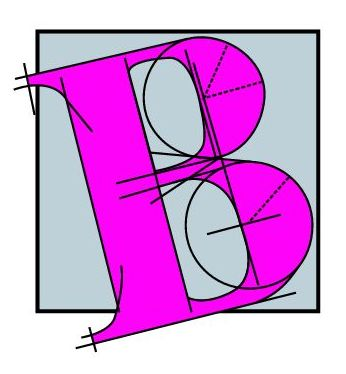
\includegraphics[width=\textwidth]{D:/Dropbox/enseignement/CPGE/raphaelpoiree/paquets/logoBaggio.jpg}
\end{center}
\end{minipage}
\begin{minipage}{0.8\linewidth}
\begin{center}
\vspace{0.2cm}

\large{\MakeUppercase{\partie}}\\

\vspace{0.2cm}

\huge{
Cours \numero \ - \titre
}
\end{center}
\end{minipage}
\begin{minipage}{0.1\linewidth}
\end{minipage}

\vspace{0.4cm}
\rule{\linewidth}{5pt}

\end{center}

\begin{center}
\MakeUppercase{\etablissement} - \MakeUppercase{\auteur} - \MakeUppercase{\classe} - \MakeUppercase{\annee}
\end{center}

\tableofcontents
%\minitoc

%\vfill

%\vspace{1cm}
\ifthenelse{\boolean{version_prof}}{

\ifthenelse{\boolean{version_kara}}{
		\begin{bclogo}[couleur = red!70,logo=\bcpanchant]{À faire}
		\begin{itemize}
		\afaire
		\end{itemize}
		\end{bclogo}
		}{} %fin ifthenelse version kara

		\begin{bclogo}[couleur = green!30,logo=\bcoutil]{Pré-requis}
		\begin{itemize}
		\prerequis
		\end{itemize}
		\end{bclogo}
\begin{minipage}{0.5\textwidth}
		\begin{bclogo}[couleur = yellow!30,logo=\bctrombone]{Connaissances}
		\begin{itemize}
		\connaissances
		\end{itemize}
		\end{bclogo}
\end{minipage}
\begin{minipage}{0.5\textwidth}
		\begin{bclogo}[couleur = yellow!30,logo=\bctrombone]{Savoir-faire}
		\begin{itemize}
		\savoirfaire
		\end{itemize}
		\end{bclogo}
\end{minipage}

		\begin{bclogo}[couleur = white!30,logo=\bccalendrier]{Organisation}
		\begin{itemize}
		\organisation
		\end{itemize}
		\end{bclogo}
		}{}
%	 \lhead{\MakeUppercase{\partie}}
%    \chead{Cours \numero}
%    \rhead{\titre}
%    \lfoot{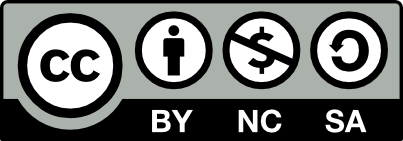
\includegraphics[width=1.2cm]{paquets/Creative_Commons.png} \hspace{0.1cm} \etablissement - \auteur\\ \ }
%    \cfoot{\thepage/\pageref{LastPage}}
%    \rfoot{Version \version - \classe}
%    \renewcommand{\headrulewidth}{0.2pt}
%    \renewcommand{\footrulewidth}{0.2pt}	
}%% Fin mode article

%%%%%%%%%%%%%%%%%%%%%%%%%  MODE PRÉSENTATION %%%%%%%%%%%%%%%%%%%%%%%%%%%%%%%%%%%

\mode<presentation>{
\title{Cours \numero \ - \titre}
\date{Version \version \  du \today}
\author{\auteur}
\institute{\etablissement -  \classe}

%%%%% PREMIÈRE SLIDE
\begin{frame}

	\begin{center}
		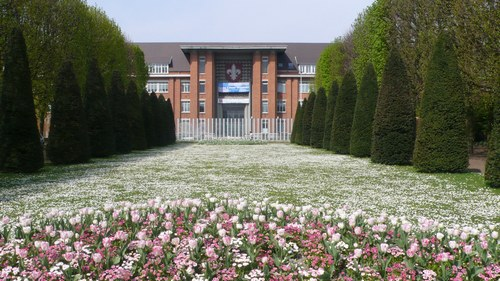
\includegraphics[height=3cm]{img/bandeau_1}
	\end{center}


	\maketitle

\end{frame}



\ifthenelse{\boolean{version_prof}}{
\begin{frame}[allowframebreaks]\titreslide{Informations professeur}
		\ifthenelse{\boolean{version_kara}}{
		\begin{bclogo}[couleur = red!70,logo=\bcpanchant]{À faire}
		\begin{itemize}
		\afaire
		\end{itemize}
		\end{bclogo}}{}

		
		\begin{bclogo}[couleur = white!30,logo=\bccalendrier]{Organisation}
		\begin{itemize}
		\organisation
		\end{itemize}
		\end{bclogo}
\end{frame}}{}
}%% Fin mode présentation
}{}%% Fin version cours

%% Version EXO

\ifthenelse{\boolean{Exo}}{
\title{Exercices}
\mode<article>{
	\lhead{\MakeUppercase{\partie}}
%    \chead{Exercice \numero}
    \rhead{Exercices}
    \lfoot{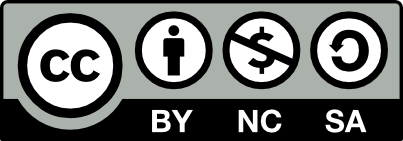
\includegraphics[width=1.2cm]{paquets/Creative_Commons.png} \hspace{0.1cm} \etablissement - \auteur }
    \cfoot{\thepage/\pageref{LastPage}}
    \rfoot{Version \version}
    \renewcommand{\headrulewidth}{0.2pt}
    \renewcommand{\footrulewidth}{0.2pt}
    }% Fin mode article	
\mode<presentation>{
\maketitle
}
}{}%% Fin version exercice


\ifthenelse{\boolean{TD}}{
\title{TD \numero}
\mode<article>{
}% Fin mode article	
\mode<presentation>{
\maketitle
}
}{}%% Fin version TD


\section{Introduction}
\begin{frame}\titreslide{Système d'ouverture de porte de TGV}
\source{Source à retrouver}

On considère 3 bases \baseB{0}, \baseB{1} et \baseB{2} telles que :
\begin{itemize}
	\item \baseB{1} est en rotation d'angle $\alpha$ par rapport à \baseB{0} autour de $\vz{0}=\vz{1}$,
	\item \baseB{2} est en rotation d'angle $\theta$ par rapport à \baseB{1} autour de $\vy{1}=\vy{2}$,
\end{itemize}

\question{Représenter les forces agissant sur la barre}
\reponse{Ceci est le déroulement de la réponse. \resultat{Ceci est le résultat...}}
\end{frame}


\section{Système d'ouverture de porte de TGV}

\begin{frame}\titreslide{Système d'ouverture de porte de TGV}
\source{Adapté de Centrale-Supelec MP 2008 par Florestan Mathurin}
\begin{minipage}{0.4\textwidth}
La figure de droite montre l'interface assurant, à partir des informations délivrées par l'unité centrale de commande, la fermeture hermétique et le verrouillage d'une porte de TGV
\end{minipage}

L’ordre de fermeture de la porte est donné soit par appui sur le bouton situé sur la porte soit via un ordre fourni par le conducteur du TGV depuis son pupitre. L’information est traitée par l’unité centrale qui pilote un moteur électrique permettant, dans un premier temps, de fermer la porte grâce à un mécanisme pignon-crémaillère puis, dans un deuxième temps, lorsque la position de fermeture est détectée, de verrouiller la porte. La détection de la position fermée enclenche également le gonflage des joints assurant l’herméticité de la fermeture. L’information de fin d’opération est transmise au conducteur sur son pupitre. 

\question{Réaliser le diagramme de définition du bloc du système.}
\reponse{Proposition de bdd possible :}
\question{Lister les composants appartenant à la chaîne d'information et les composants appartenant à la chaîne d'énergie.}
\end{frame}
\end{document}